\documentclass[a4paper]{article}
\usepackage[utf8]{inputenc}
\usepackage{graphicx}
\usepackage[backend=biber, style=nature]{biblatex}
\usepackage{gensymb}
\usepackage{textcomp}
\usepackage{pdfpages}
\addbibresource{references.bib}

\newcommand{\delO}[1]{\ensuremath{\mathrm{\delta ^{18}O_{#1}}}} % delta-18-O symbol
\newcommand{\textapprox}{\raisebox{0.5ex}{\texttildelow}} % centred tilde
\newcommand{\fC}{$^{14}\mathrm{C}$} % carbon-14
\newcommand{\BP}{$\mathrm{\Delta}^{14}\mathrm{C}_{\mathrm{B-P}}${}} % delta-14-C B-P
\newcommand{\eNd}{$\mathrm{\epsilon}$Nd} % epsilon neodymium
\newcommand{\PaTh}{$^{231}$Pa/$^{230}$Th} % Pa/Th

\begin{document}

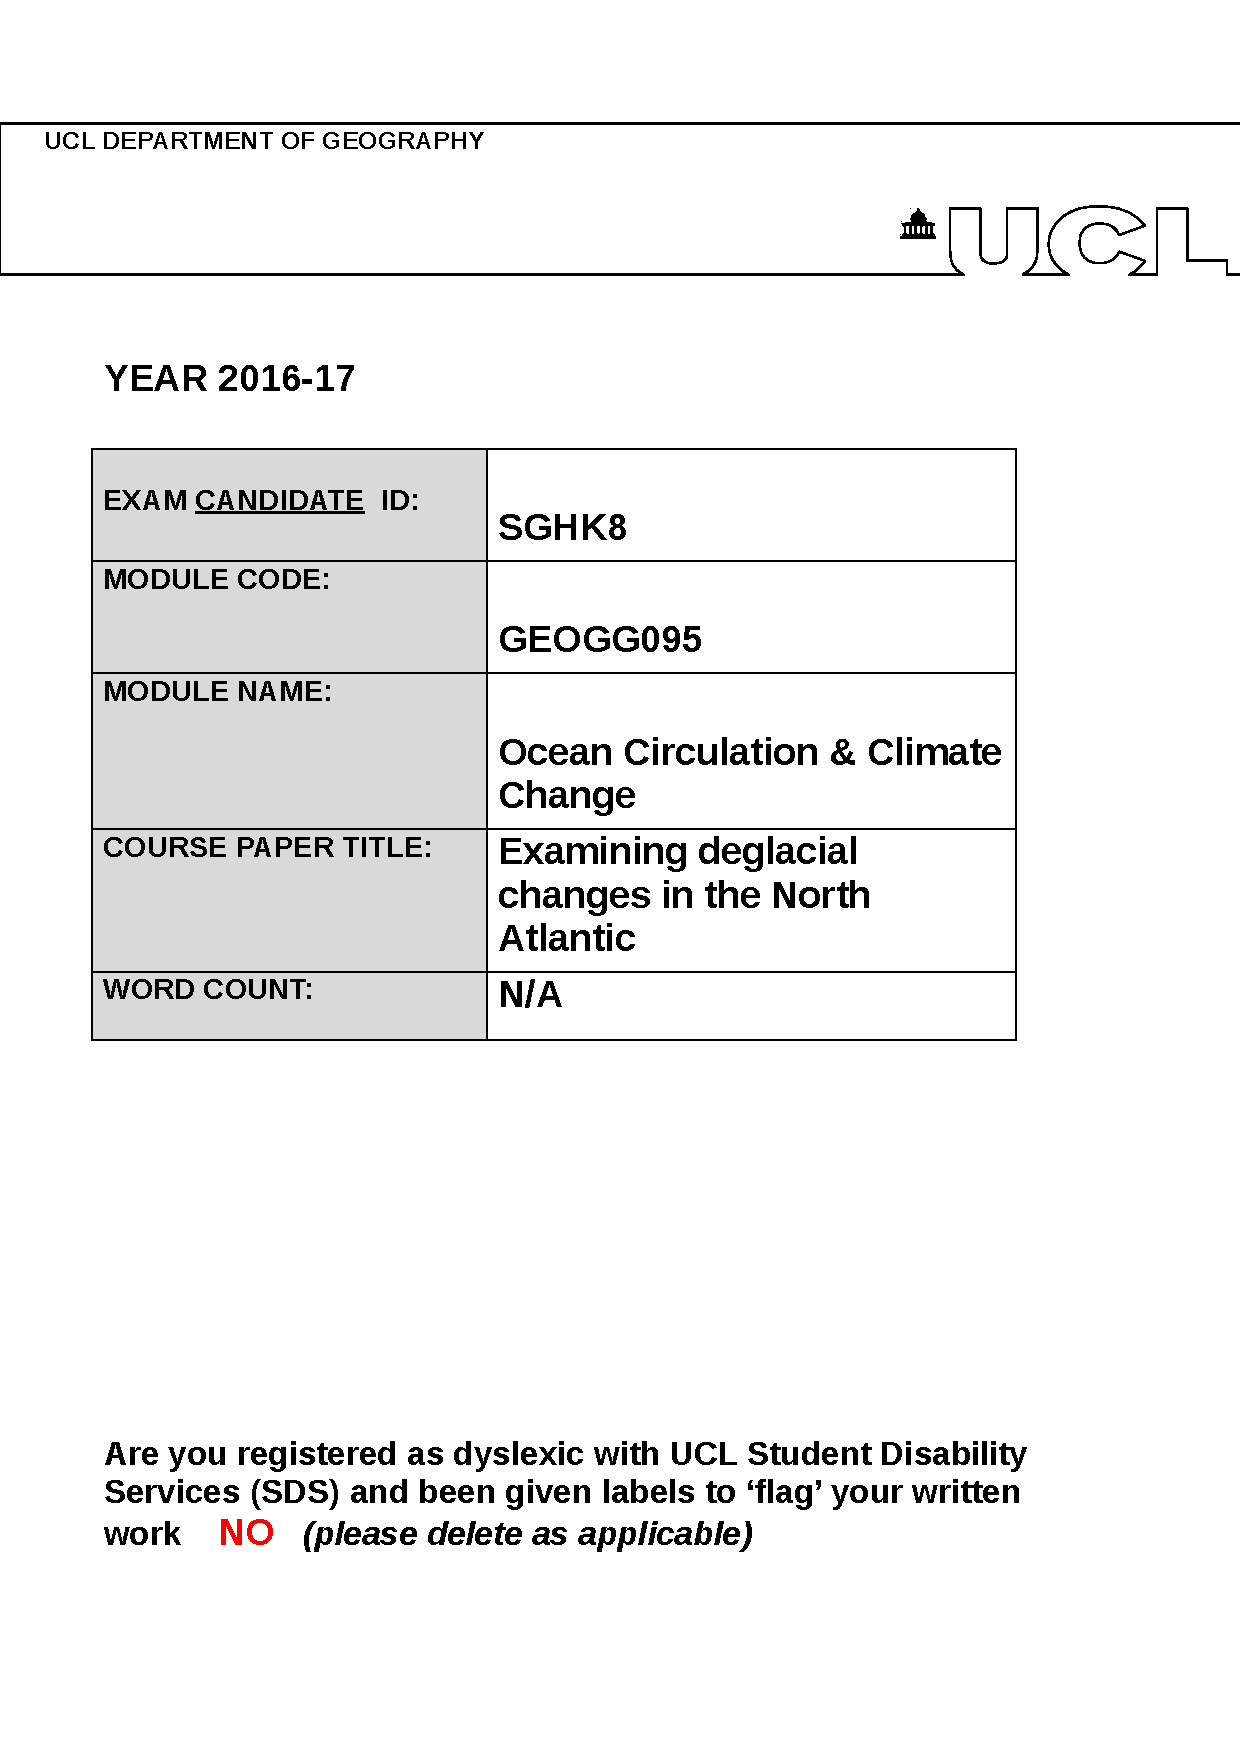
\includepdf{coursework-submission-coversheet.pdf}

\title{Examining deglacial circulation in the North Atlantic}
\author{SGHK8}
\date{}
\maketitle

\section{Exercise 1 - Mid-depth temperature and \delO{SW} reconstruction}

\subsection{Question 1}
\label{sec:Q1}
According to \citeauthor{barker2003study} \parencite{barker2003study}, foraminiferal Fe/Mg molar ratios greater than approximately 0.1 are indicative of potential contamination by Mg-rich clay silicates.
Mg/Ca measurements could therefore be rejected if they do not meet the criteria:

\begin{equation} \label{eq:fe_mg}
    \frac{\mathrm{Fe}/\mathrm{Ca}}{\mathrm{Mg}/\mathrm{Ca}} < 0.1 \, \mathrm{mol \cdot mol^{-1}}
\end{equation}

However, visual assessment of the magnitude of potential contamination (Figure \ref{fig:Mg_Fe}) shows that all but one of the eight measurements failing the this criteria are close to the rest of the data in terms of Fe/Mg.
As a result, only the 16.39 ka measurement labelled in Figure \ref{fig:Mg_Fe} is rejected for contamination.

\begin{figure}[h]
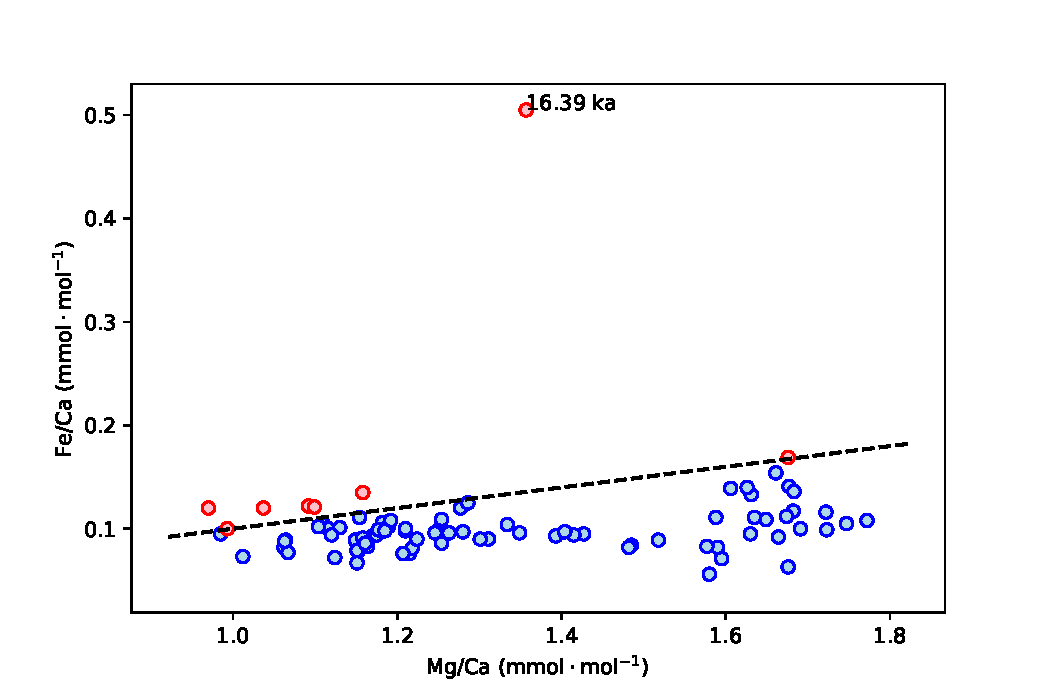
\includegraphics[width=\textwidth]{img/scatter_MgCa_x_FeCa_contaminated.pdf}
    \caption{Ratio of Mg/Ca to Fe/Ca in benthic foraminifera \emph{M. barleeanuum} in RAPiD-10-1P sediment core.
             Dashed line seperates potentially contaminated measurements (red points) according to Equation \ref{eq:fe_mg}.
             Labelled point is identified for rejection.}
        \label{fig:Mg_Fe}
\end{figure}

\subsection{Question 2}
As shown in Figure \ref{eq:timeseries}, the bottom water oxygen isotope excursion \delO{SW} declines to negative values after the Last Glacial Maximum (LGM) in correspondance with falling bottom water temperatures.
The two trends fall sharply toward the beginning of Heinrich Stadial 1 (HS1) before diverging: in contrast to the gradual temperature recovery from nearly 0 \degree{}C, \delO{SW} continues to strongly decrease until the transition into the Bølling–Allerød warm period (BA, 14.7–12.9 ka \parencite{thornalley2011reconstructing}), at which point both lines rise together rapidly.
The Younger Dryas (YD) marks a very abrupt return to HS1 temperatures, although the concurrent drop in \delO{SW} is not as severe, whereas each record shows relative stability over the course of the Holocene.

The imprint of local salinity on foramineferal Mg/Ca may result in significant systematic positive bias in reconstructed \delO{SW} \parencite{mathien2009salinity}, whereas uncertainties in foramineferal \delO{carbonate} stemming from nonclimatic factors, such as measurement imprecision or variations in seawater carbonate ion concentration, are comparatively small \parencite{bell2014local}. 
Assuming these issues are negligeable, the dominant control of surface water oxygen isotopic composition by the precipitation/evaporation/freshwater input balance --- i.e. salinity --- make \delO{SW} an effective indicator of the source of the ocean water mass \parencite{ravelo2007use, lynch2014tracers}. 

% Do the abrupt drops in delO{SW} and temperature preceeding HS1 confirm input of meltwater from a Heinrich event?

\begin{figure} \label{eq:timeseries}
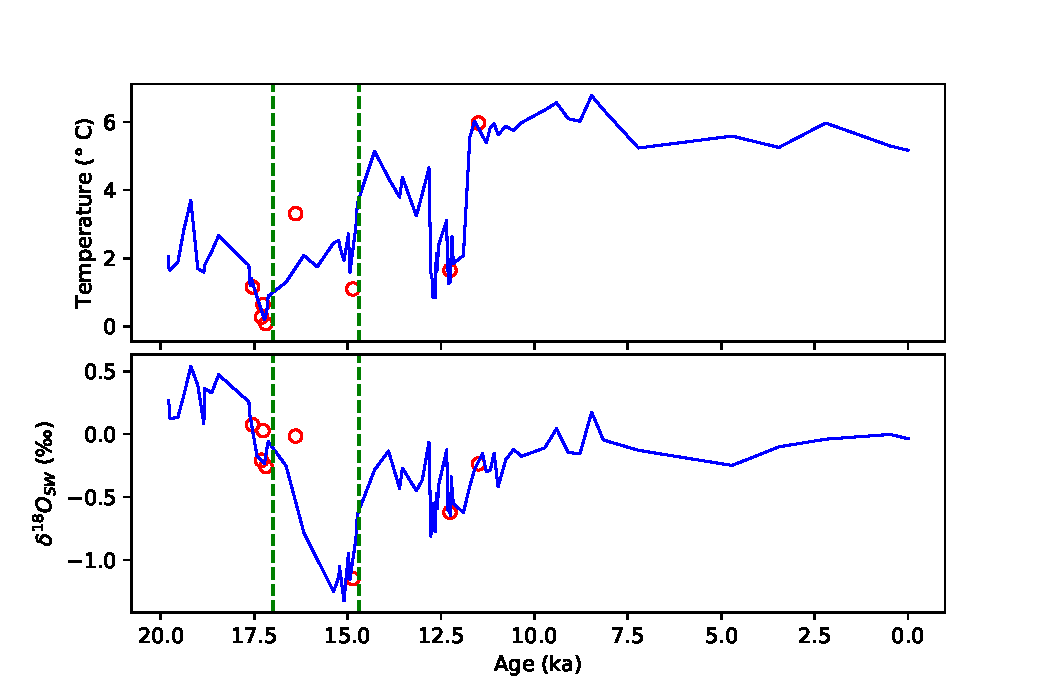
\includegraphics[width=\textwidth]{img/timeseries_temp_and_d18Osw.pdf}
    \caption{Trends in the ice-volume corrected \delO{SW} (top) and bottom water temperature since the Last Glacial Maximum determined from Mg/Ca palaeothermetry (bottom) recorded in RAPid-10-1P.
             Red points and the gap in the timeseries signify a rejected measurement (see text in Section \ref{sec:Q1}).
             Shaded regions mark Heinrich Stadial 1 (HS1) and Younger Dryas (YD), as defined in \citeauthor{thornalley2011reconstructing} \parencite{thornalley2011reconstructing}}.
        \label{fig:timeseriestempd18Osw}
\end{figure}

\section{Exercise 2: Tracers of deep ocean circulation change}
\label{sec:E2}

\subsection{Question 1}
\label{sec:Q2.1}
See Figure \ref{fig:age_depth}

\begin{figure}[!htbp]
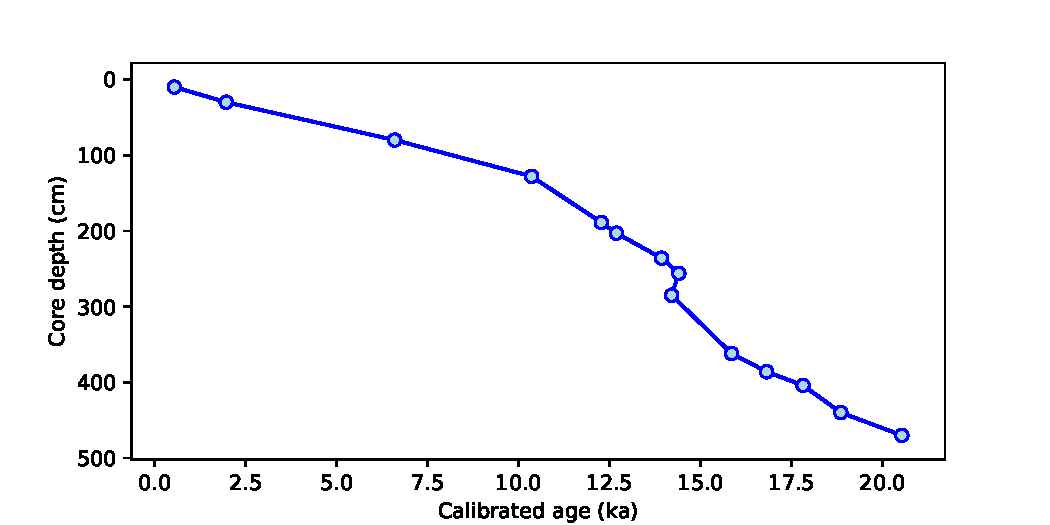
\includegraphics[width=\textwidth]{img/line_age_depth.pdf}
    \caption{Planktic foraminifera calibrated age against depth in sediment core OCE-326-GGC14, on the Laurentian fan.}
        \label{fig:age_depth}
\end{figure}

\subsection{Question 2}
\label{sec:Q2.2}

\begin{figure}[!htbp]
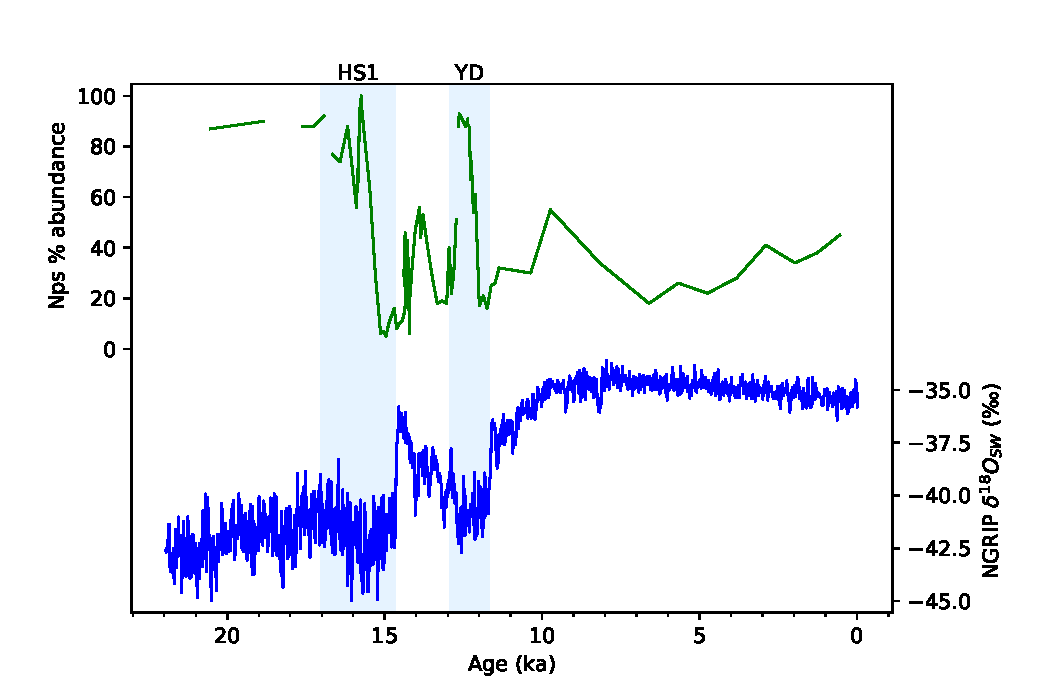
\includegraphics[width=\textwidth]{img/timeseries_nps_ngrip}
    \caption{Time series of abundance of planktic foraminifera \emph{N. pachyderma} sinistral (\emph{Nps}) in OCE-326-GGC14 (top) and oxygen isotope excursion in Greenland ice core NGRIP (bottom).}
        \label{fig:nps_ngrip}
\end{figure}

Figure \ref{fig:nps_ngrip} shows a strong antiphase relationship between \emph{Nps} abundance in the North Atlantic and \delO{} in Greenland, and both record abrupt climate cooling during the HS1 and YD stadials.
While changes in the latter appear to lag those in the former by approximately 0.5--1 ka, there is uncertainty in the calibration of foraminiferal \fC{} radiocarbon dates due to measurement error and, in particular, the assumption of a constant 400 year radiocarbon reservoir age --- a value that was likely higher during stadial events due to decreased ocean ventilation \parencite{bard1994north, hughen2004marine04}.

            
\subsection{Question 3}
\label{sec:Q2.3}
\begin{figure}[p]
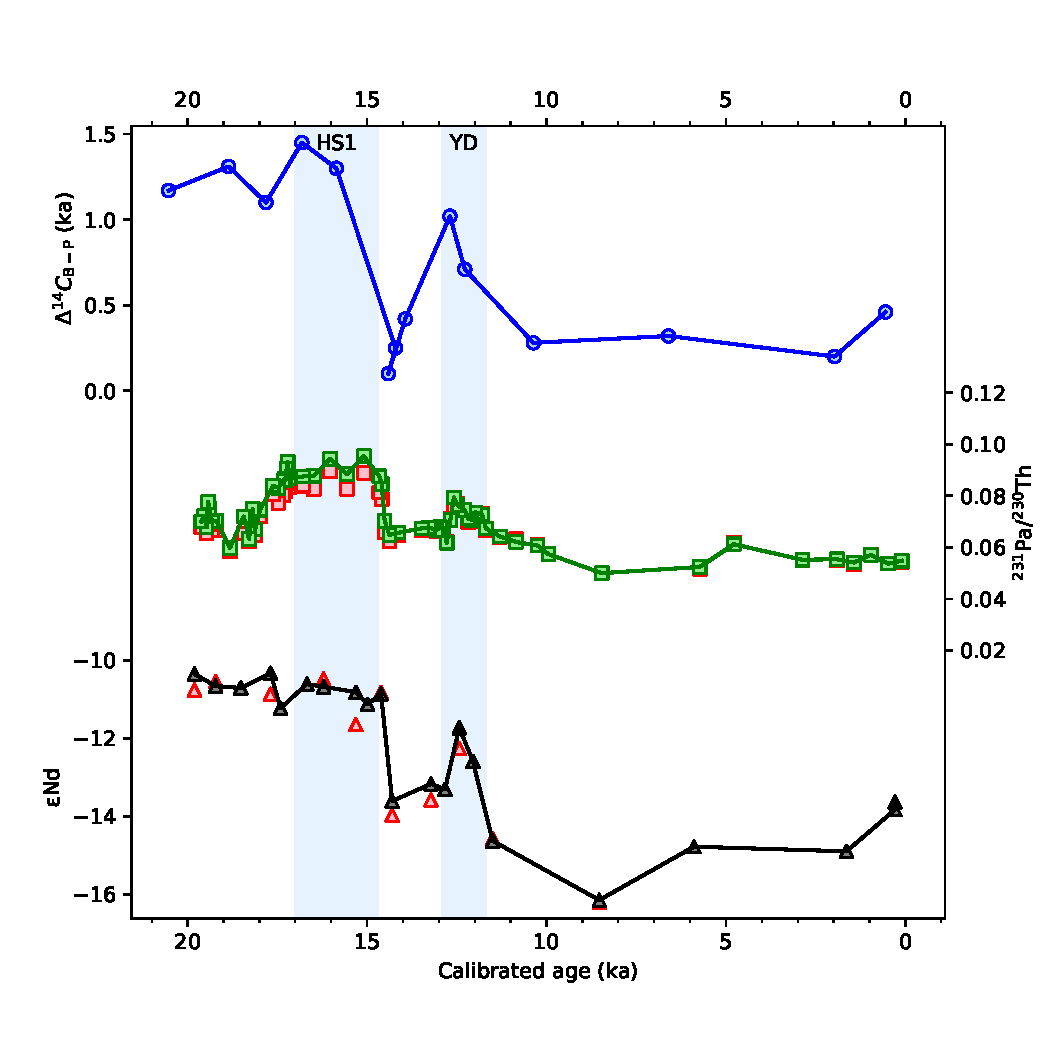
\includegraphics[width=\textwidth]{img/timeseries_B-P_PaTh_eNd}
    \caption{Time series of benthic--planktic foraminifera \fC{} ventilation age difference in OCE-326-GGC14 (top);
             \PaTh{} ratio in calculated against $^{238}$U (green) and $^{232}$U (red) OCE326-GGC5 core on Bermuda rise \parencite[data from][]{mcmanus2004collapse};
             Neodynium isotopic ratio excursion in unclean foraminifera (black) and reductively cleaned fish debris (red) from OCE326-GGC6 sediment core on Bermuda Rise (bottom) \parencite[data from][]{roberts2010synchronous}.}
            \label{fig:bp_path_end}
\end{figure}
The benthic--planktic foraminifera \fC{} offset (Figure \ref{fig:bp_path_end}, top) is considerably larger at LGM, HS1 and YD than during the BA and the Holocene.
Since \BP{} of a water mass effectively records the ventilation age (i.e. time since last exposure at the surface) \parencite{lynch2014tracers}, these results indicate that the North Atlantic was highly stratified during the cold periods, with younger northern sourced waters displaced in the deep ocean by the intrusion of more ancient waters of southern origin.
This supports evidence for the slowdown or shutoff of NADW formation during these cold periods, allowing Antarctic Bottom Water to fill the global abyssal basins \parencite{boyle1985comparison, bard1994north, thornalley2011deglacial}.
Likewise, the rapid rejuvenation of deep waters at the HS1--BA and YD--Holocene transitions shown in the \BP{} time series indicates rapid resumption of the contemporary (warm) mode ocean overturning circulation.

\subsection{Question 4}
\label{sec:Q2.4}
The \BP{} changes described in Section \ref{sec:Q2.3} are largely consistent with isotopic trends described in other studies, as depicted in Figure \ref{fig:bp_path_end}.
The ratio of $^{231}$P sequestered in marine sediments to the more quickly scavenged $^{230}$Th is an indicator of the residence time of the overlying water mass \parencite{lynch2014tracers}, and the high values recorded on the Bermuda rise for the HS1, and to a lesser extent YD, indicate poor export of $^{231}$P from the region during the postglacial stadials.
This can be explained by the arrest of the southward movement of NADW, as described above, with the steep \PaTh{} drop at \textapprox 15.5 marking the abrupt resumption of the AMOC following HS1 \parencite{mcmanus2004collapse}.
However, one issue with this using the sedimentary \PaTh{} signal to infer changes in global circulation is that the distinction between a complete shutdown and a more moderate shift to a shallower, more locally confined circulation of North Atlantic waters is not always readily apparent, since it essentially records change in the entire column of water above \parencite{roberts2010synchronous}. 
Since \eNd{} serves as a form of water mass signature, it can be used to supplement the interpretation of the other records in Figure \ref{fig:bp_path_end} \parencite{lynch2014tracers}. 
The high values from the LGM through to the end of HS1 provide evidence for the incursion of AABW into the Northwest Atlantic, with a marked shift to less radiogenic Northern-sourced waters following the YD, supporting the theory of AMOC modulation as a distinctive feature of deglacial climate change \parencite{roberts2010synchronous}.

\newpage
\printbibliography{}
\end{document}
